\section{Sparse vs. Dense Models: Trade‑offs & Motivations}
\begin{frame}[allowframebreaks]{}
    \LARGE Sparse vs. Dense Models: \textbf{Trade‑offs & Motivations}
\framebreak
    \begin{figure}[h]
        \centering
        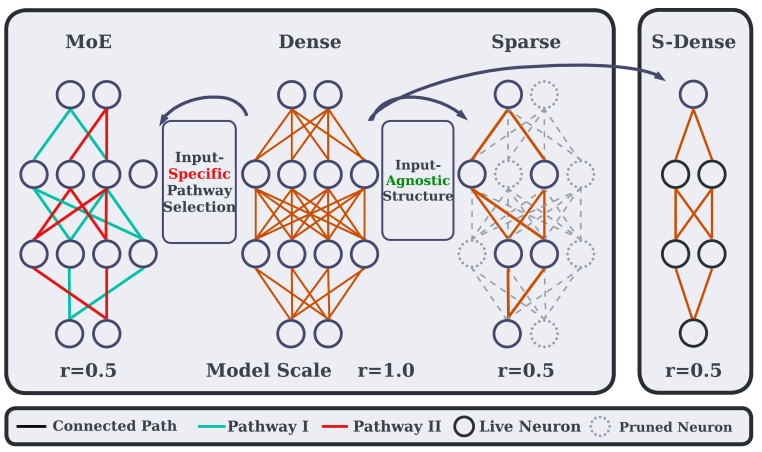
\includegraphics[width=\textwidth,height=0.84\textheight,keepaspectratio]{images/lrm+moe/dense_sparse.png}
        \caption*{Source: \href{https://arxiv.org/abs/2308.10110}{Zhang et al. (2023)}}
        % \fetchconvertimage{https://blog.reachsumit.com/img/posts/2023/generative-retrieval/sparse_vs_dense_retrieval.png}{images/lrm+moe/sparse+dense.png}{width=\textwidth,height=0.9\textheight,keepaspectratio}
    \end{figure}
\end{frame}

\begin{frame}[allowframebreaks]{Sparse vs. Dense Models: Trade‑offs & Motivations}
    \begin{itemize}
        \item \textbf{Dense Models:}
        \begin{itemize}
            \item Use a large number of parameters.
            \item All parameters participate for every input.
            \item Compute cost is predictable and uniform.
            \item Training is straightforward—no need for routing or selection.
            \item Require more computational resources.
            \item \textbf{Examples:}
            \begin{itemize}
                \item Standard Transformer models (e.g., BERT, GPT).
                \item Fully-connected neural networks.
            \end{itemize}
        \end{itemize}
    \framebreak
        \item \textbf{Sparse Mixture-of-Experts (MoE) Models:}
        \begin{itemize}
            \item Only a subset (top-$k$) of experts are activated per input.
            \item Enables scaling to billions of parameters without increasing per-token compute.
            \item Requires a routing mechanism to select experts.
            \item Focus on specific features or patterns in the data.
            \item Efficient for large datasets with sparse representations.
            \item \textbf{Examples:}
            \begin{itemize}
                \item Switch Transformer (Google).
                \item GLaM (Google).
                \item M6-T (Alibaba).
            \end{itemize}
        \end{itemize}
    \framebreak
        \begin{figure}[h]
            \centering
            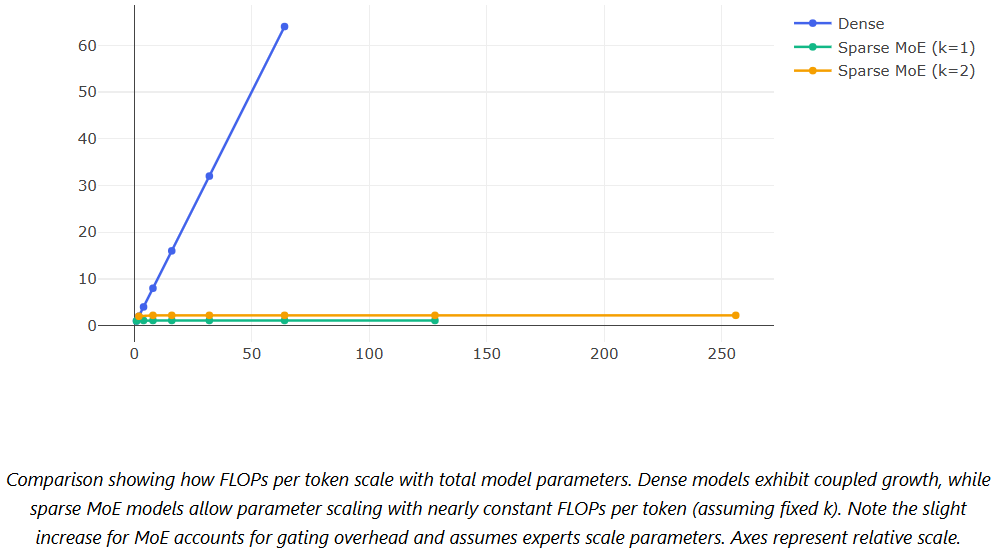
\includegraphics[width=\textwidth,height=0.8\textheight,keepaspectratio]{images/lrm+moe/dense_sparse_flops.png}
            \caption*{Source: \href{https://apxml.com/courses/mixture-of-experts/chapter-1-moe-foundations-sparse-models/dense-vs-sparse-activation}{Contrasting Dense vs. Sparse Activation}}
        \end{figure}
    \framebreak
        \item \textbf{Trade-offs:}
        \begin{itemize}
            \item \textbf{Dense:} Simpler, stable, but limited by compute and memory.
            \item \textbf{Sparse:} Higher capacity, efficient compute, but adds routing overhead.
            \item Sparse models may face instability and load balancing issues.
            \item Choice depends on scale, task complexity, and infrastructure.
        \end{itemize}
    \end{itemize}
\end{frame}